\documentclass[12pt]{article}
\usepackage[english]{babel}
\usepackage[utf8x]{inputenc}
\usepackage{amsmath}
\usepackage{tikz}
\usetikzlibrary{arrows,automata}
\begin{document}
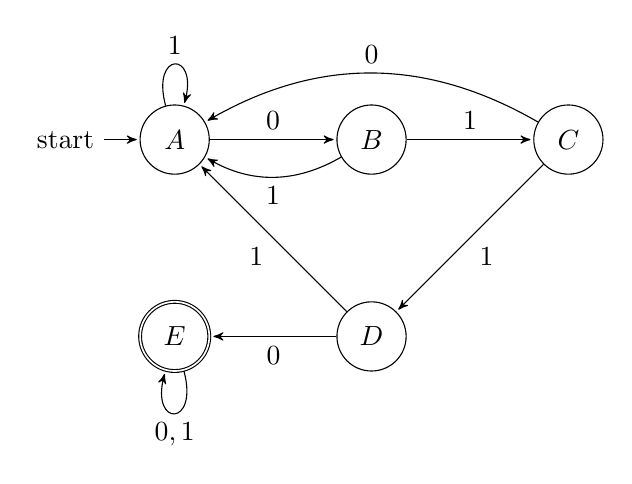
\begin{tikzpicture}[->,>=stealth',shorten >=1pt,auto,node distance=2.5cm,
        scale = 1,transform shape]

  \node[state,initial] (A) {$A$};
  \node[state] (B) [right of=A] {$B$};
  \node[state] (C) [right of=B] {$C$};
  \node[state] (D) [below of=B] {$D$};
  \node[state,accepting] (E) [left of=D] {$E$};

  \path (A) edge    node {$0$} (B)
        (A) edge[loop above]    node {$1$} (A)
        (B) edge[bend left, below]    node {$1$} (A)
        (C) edge[bend right, above]    node {$0$} (A)
        (D) edge    node {$1$} (A)
        (B) edge    node {$1$} (C)
        (C) edge    node {$1$} (D)
        (D) edge    node {$0$} (E)
        (E) edge[loop below]    node {$0,1$} (E);

\end{tikzpicture}

\vspace{3cm}

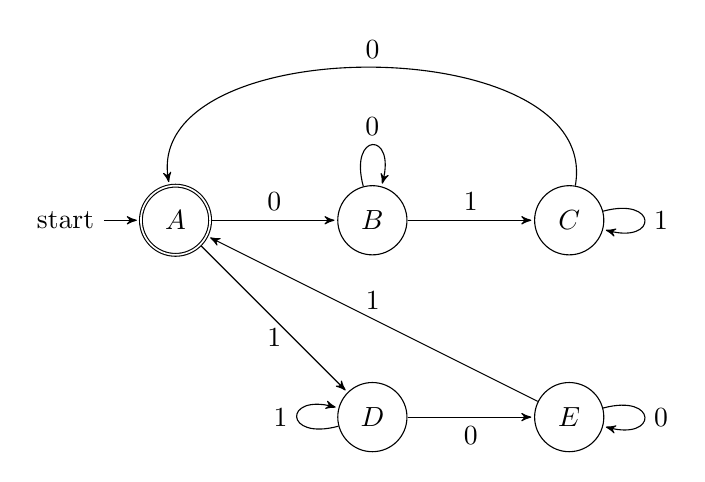
\begin{tikzpicture}[->,>=stealth',shorten >=1pt,auto,node distance=2.5cm,
  scale = 1,transform shape]

\node[state,initial,accepting] (A) {$A$};
\node[state] (B) [right of=A] {$B$};
\node[state] (C) [right of=B] {$C$};
\node[state] (D) [below of=B] {$D$};
\node[state] (E) [right of=D] {$E$};

\path 
  (A) edge node {$0$} (B)
  (B) edge node {$1$} (C)
  (C) edge[bend right=100, above] node {$0$} (A)
  (A) edge[below] node {1} (D)
  (D) edge[below] node {0} (E)
  (E) edge[above] node {1} (A)
  (B) edge[loop above] node{0} (B)
  (C) edge[loop right] node{1} (C)
  (D) edge[loop left] node{1} (D)
  (E) edge[loop right] node{0} (E)
  % (A) edge[loop above]    node {$1$} (A)
  % (B) edge[bend left, below]    node {$1$} (A)
  % (C) edge[bend right, above]    node {$0$} (A)
  % (D) edge    node {$1$} (A)
  % (B) edge    node {$1$} (C)
  % (C) edge    node {$1$} (D)
  % (D) edge    node {$0$} (E)
  % (E) edge[loop below]    node {$0,1$} (E)
  ;

\end{tikzpicture}
\end{document}
